\documentclass{article}
\usepackage{amsmath}
\usepackage{tikz}
\usetikzlibrary{arrows.meta}

\begin{document}

\begin{center}
    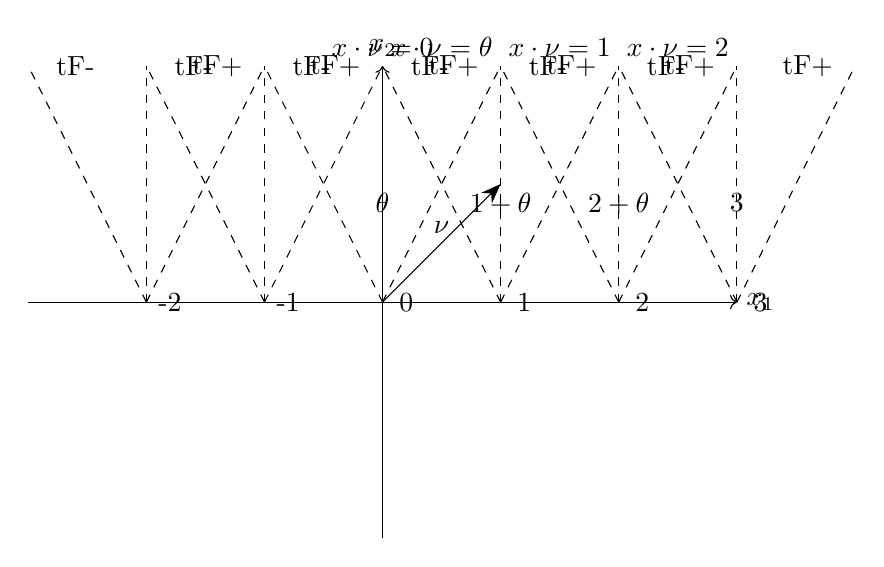
\begin{tikzpicture}[scale=1.5]
        % Axes
        \draw[->] (-3,0) -- (3,0) node[right] {$x_1$};
        \draw[->] (0,-2) -- (0,2) node[above] {$x_2$};

        % Lines representing different values of x . ν
        \foreach \x/\label in {-2/-2, -1/-1, 0/0, 1/1, 2/2, 3/3} {
            \draw[dashed] (\x,0) -- (\x,2);
            \node at (\x+.2,0) {\label};
        }

        % Lines representing tF+
        \foreach \x/\label in {-2/-2, -1/-1, 0/0, 1/1, 2/2, 3/3} {
            \draw[dashed] (\x,0) -- (\x+1,2);
            \node at (\x+.6,2) {tF+};
        }

        % Lines representing tF-
        \foreach \x/\label in {-2/-2, -1/-1, 0/0, 1/1, 2/2, 3/3} {
            \draw[dashed] (\x,0) -- (\x-1,2);
            \node at (\x-.6,2) {tF-};
        }

        % Vector ν
        \draw[-{Stealth[scale=1.5]}] (0,0) -- (1,1) node[midway, above] {$\nu$};

        % Text annotations
        \node at (0,2) [above] {$x \cdot \nu = 0$};
        \node at (.5,2) [above] {$x \cdot \nu = \theta$};
        \node at (1.5,2) [above] {$x \cdot \nu = 1$};
        \node at (2.5,2) [above] {$x \cdot \nu = 2$};
        \node at (0,1) [below] {$\theta$};
        \node at (1,1) [below] {$1+\theta$};
        \node at (2,1) [below] {$2+\theta$};
        \node at (3,1) [below] {$3$};
    \end{tikzpicture}
\end{center}

\textbf{Deformation gradient for oscillating solutions, $F_+ = F_0 + a \otimes \nu$, $F_- = F_0 + b \otimes \nu$.}

\end{document}